%!TEX root = hard_stack_paper/paper.tex

\begin{figure*}[t]
\begin{subfigure}[t]{\textwidth}
\centering
\scalebox{0.72}{%
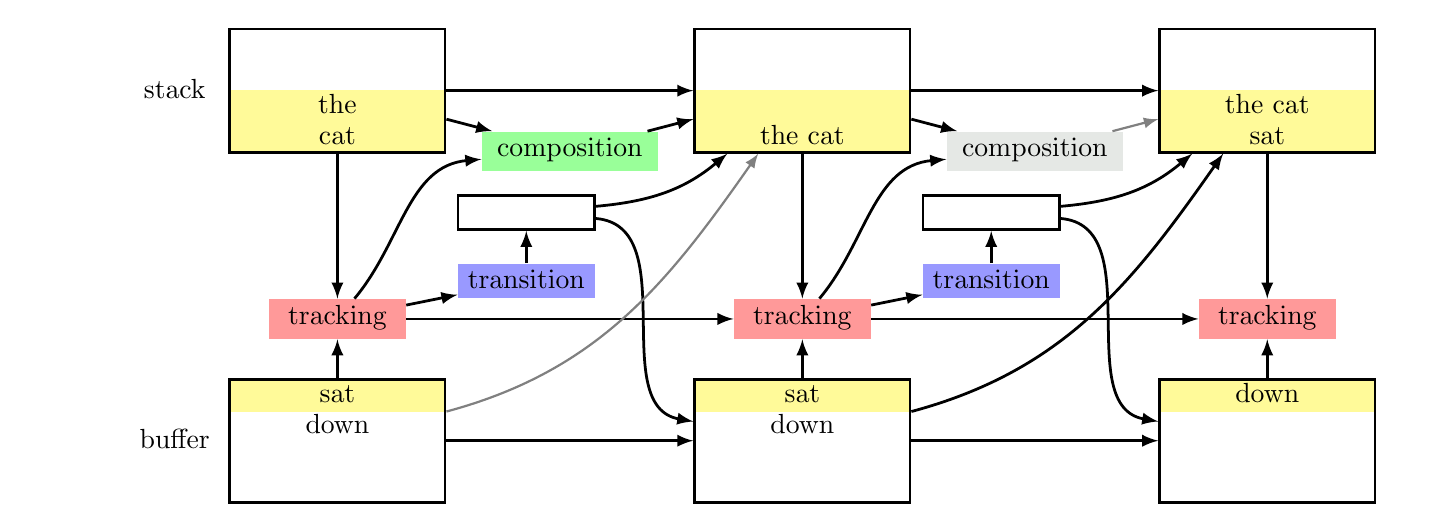
\begin{tikzpicture}
    \def\dx{21pt}
    \def\dy{11pt}
    \def\sy{12*\dy}
    \def\oxb{8*\dx}
    \def\by{0pt}
    \def\ox{0*\oxb}

    \tikzstyle{label}=[text width=35mm,align=center,text height=2mm]    
    \tikzstyle{word}=[text width=35mm,align=center,text height=2mm]    
    \tikzstyle{tracker}=[fill=red!40,text width=15mm,align=center,text height=2mm]
    \tikzstyle{softmax}=[fill=blue!40,text width=15mm,align=center,text height=2mm]
    \tikzstyle{comp}=[fill=green!40,text width=20mm,align=center,text height=2mm]
    \tikzstyle{compoff}=[fill=green!10!black!10,text width=20mm,align=center,text height=2mm]
    \tikzstyle{result}=[line width=1pt,draw=black,text width=15mm,align=center,text height=2mm]    
    \tikzstyle{sbox}=[line width=1pt,draw=black,text width=25mm,align=center,text height=13.3mm]
    \tikzstyle{bbox}=[line width=1pt,draw=black,text width=25mm,align=center,text height=13.3mm]
    \tikzstyle{focus1}=[fill=yellow!40,text width=25mm,align=center,text height=2mm]
    \tikzstyle{focus2}=[fill=yellow!40,text width=25mm,align=center,text height=5.5mm]

    \node[label]  (sl) at (\ox-0.35*\oxb+0*\dx,\by+1*\dy) {buffer};

    \node[focus1] (0bb) at  (\ox+0*\dx,2.5*\dy) {};
    \node[word]  (0b3) at (\ox+0*\dx,\by-0.5*\dy) {};
    \node[word]  (0b2) at (\ox+0*\dx,\by+1.5*\dy) {down};
    \node[word]  (0b1) at (\ox+0*\dx,\by+2.5*\dy) {sat};
    \node[bbox] (0bb) at  (\ox+0*\dx,\by+1.0*\dy) {};
    
    \node[label]  (sl) at (\ox-0.35*\oxb+0*\dx,\sy+0.5*\dy) {stack};
    
    \node[focus2] (0sb) at  (\ox+0*\dx,\sy-0.5*\dy) {};
    \node[word]  (0s1) at (\ox+0*\dx,\sy-1*\dy) {cat};
    \node[word]  (0s2) at (\ox+0*\dx,\sy+0*\dy) {the};
    \node[word]  (0s3) at (\ox+0*\dx,\sy+1*\dy) {};
    \node[sbox] (0sb) at  (\ox+0*\dx,\sy+0.5*\dy) {};
    
    \node[comp] (0c) at  (\ox+0.5*\oxb,\sy-1.5*\dy) {composition};
    
    \node[tracker] (0t) at  (\ox+0*\dx,5*\dy) {tracking};
    \node[softmax] (0sm) at  (\ox+3.25*\dx,6.25*\dy) {transition};
    \node[result] (0so) at  (\ox+3.25*\dx,8.5*\dy) {\reduce};
    
    \def\ox{1*\oxb}

    \node[focus1] (1bb) at  (\ox+0*\dx,2.5*\dy) {};
    \node[word]  (1b3) at (\ox+0*\dx,\by-0.5*\dy) {};
    \node[word]  (1b2) at (\ox+0*\dx,\by+1.5*\dy) {down};
    \node[word]  (1b1) at (\ox+0*\dx,\by+2.5*\dy) {sat};
    \node[bbox] (1bb) at  (\ox+0*\dx,\by+1*\dy) {};
    
    \node[focus2] (1sb) at  (\ox+0*\dx,\sy-0.5*\dy) {};
    \node[word]  (1s1) at (\ox+0*\dx,\sy-1*\dy) {the cat};
    \node[word]  (1s2) at (\ox+0*\dx,\sy+0*\dy) {};
    \node[word]  (1s3) at (\ox+0*\dx,\sy+1*\dy) {};
    \node[sbox] (1sb) at  (\ox+0*\dx,\sy+0.5*\dy) {};
    
    \node[compoff] (1c) at  (\ox+0.5*\oxb,\sy-1.5*\dy) {composition};
    
    \node[tracker] (1t) at  (\ox+0*\dx,5*\dy) {tracking};
    \node[softmax] (1sm) at  (\ox+3.25*\dx,6.25*\dy) {transition};
    \node[result] (1so) at  (\ox+3.25*\dx,8.5*\dy) {\shift};
     
    \def\ox{2*\oxb}

    \node[focus1] (2bb) at  (\ox+0*\dx,2.5*\dy) {};
    \node[word]  (2b3) at (\ox+0*\dx,\by-0.5*\dy) {};
    \node[word]  (2b2) at (\ox+0*\dx,\by+1.5*\dy) {};
    \node[word]  (2b1) at (\ox+0*\dx,\by+2.5*\dy) {down};
    \node[bbox] (2bb) at  (\ox+0*\dx,\by+1*\dy) {};
    
    \node[focus2] (2sb) at  (\ox+0*\dx,\sy-0.5*\dy) {};
    \node[word]  (2s1) at (\ox+0*\dx,\sy-1*\dy) {sat};
    \node[word]  (2s2) at (\ox+0*\dx,\sy+0*\dy) {the cat};
    \node[word]  (2s3) at (\ox+0*\dx,\sy+1*\dy) {};
    \node[sbox] (2sb) at  (\ox+0*\dx,\sy+0.5*\dy) {};
   
    \node[tracker] (2t) at  (\ox+0*\dx,5*\dy) {tracking};

    
    \pgfsetarrowsend{latex}
    \tikzstyle{fwd} = [draw=black, line width=1pt]
    \tikzstyle{gated} = [draw=black!50, line width=0.8pt]

    \draw [fwd] (0sb) -- (0t);
    \draw [fwd] (0bb) -- (0t);
    \draw [fwd] (0t) -- (0sm);
    \draw [fwd] (0sm) -- (0so);
    \draw [fwd] (0sb) -- (0c);
    
    \draw [fwd] (0t) -- (1t);
    \draw [fwd] (0t) to[out=50,in=-175] (0c);
    \draw [fwd] (0sb) -- (1sb);
    \draw [fwd] (0bb) -- (1bb);
    \draw [fwd] (0so) to[out=5,in=-140] (1sb);
    \draw [fwd] (0so) to[out=-5,in=170] (1bb);
    \draw [gated] (0bb) to[out=15,in=-125] (1sb);
    \draw [fwd] (0c) -- (1sb);

    \draw [fwd] (1sb) -- (1t);
    \draw [fwd] (1bb) -- (1t);
    \draw [fwd] (1t) -- (1sm);
    \draw [fwd] (1sm) -- (1so);
    \draw [fwd] (1sb) -- (1c);
    
    \draw [fwd] (1t) -- (2t);
    \draw [fwd] (1t) to[out=50,in=-175] (1c);
    \draw [fwd] (1sb) -- (2sb);
    \draw [fwd] (1bb) -- (2bb);
    \draw [fwd] (1so) to[out=5,in=-140] (2sb);
    \draw [fwd] (1so) to[out=-5,in=170] (2bb);
    \draw [fwd] (1bb) to[out=15,in=-125] (2sb);
    \draw [gated] (1c) -- (2sb);

    \draw [fwd] (2sb) -- (2t);
    \draw [fwd] (2bb) -- (2t);


  \end{tikzpicture}}
  
 \caption{The SPINN model unrolled for two transitions during the processing of the sentence \word{the cat sat down}. `Tracking', `transition', and `composition' are neural network layers. Gray arrows indicate connections which are blocked by a gating function.}\label{fig:model:1d}
  
\end{subfigure}\\\\\\
\begin{subfigure}[t]{\textwidth}
\centering
\scalebox{0.5}{%
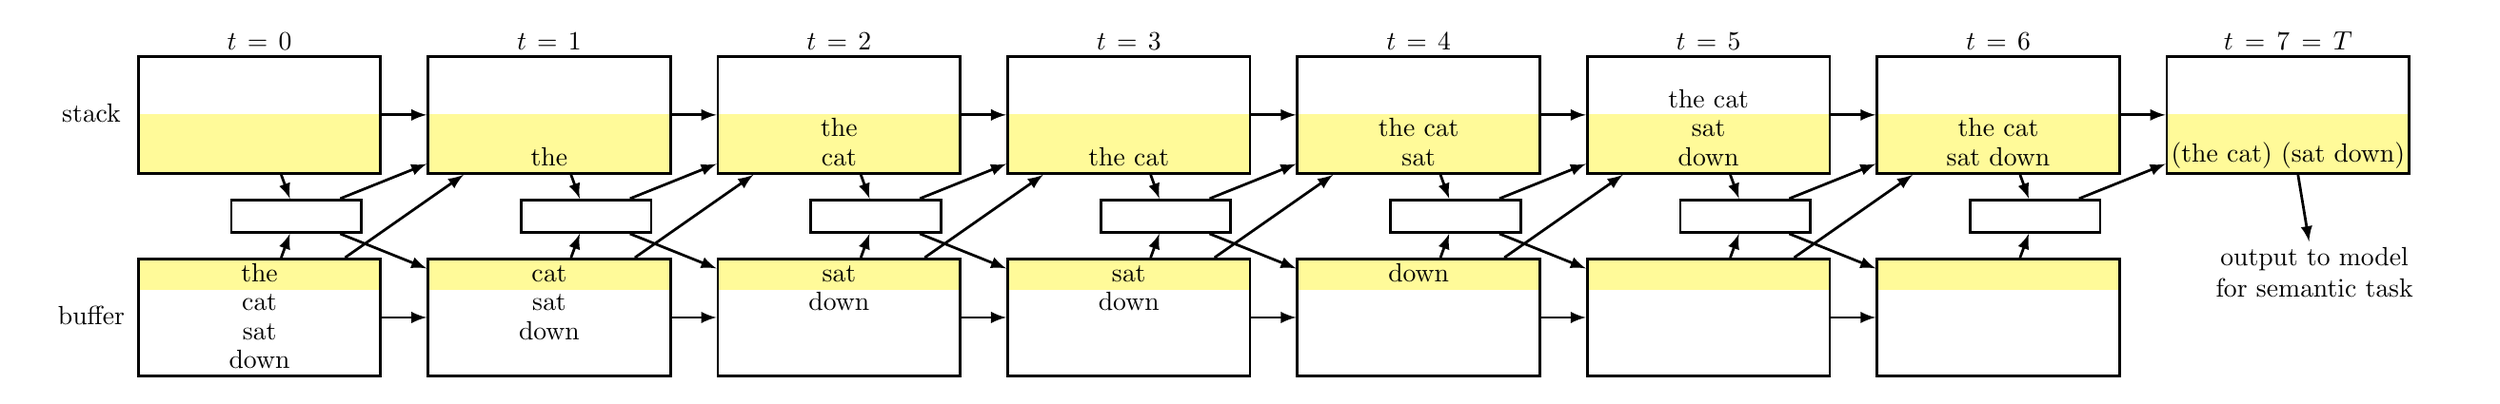
\begin{tikzpicture}
    \def\dx{20pt}
    \def\dy{11pt}
    \def\sy{7*\dy}
    \def\oxb{5.5*\dx}
    \def\by{0pt}
    \def\oxs{0pt}

    \tikzstyle{label}=[text width=15mm,align=center,text height=2mm]    
    \tikzstyle{word}=[text width=32mm,align=center,text height=2mm]    
    \tikzstyle{tracker}=[fill=red!40,text width=15mm,align=center,text height=2mm]
    \tikzstyle{softmax}=[text width=40mm,align=center,text height=2mm]
    \tikzstyle{comp}=[fill=green!40,text width=20mm,align=center,text height=2mm]
    \tikzstyle{result}=[line width=1pt,draw=black,text width=15mm,align=center,text height=2mm]    
    \tikzstyle{sbox}=[line width=1pt,draw=black,text width=30mm,align=center,text height=13.3mm]
    \tikzstyle{bbox}=[line width=1pt,draw=black,text width=30mm,align=center,text height=13.3mm]
    \tikzstyle{focus1}=[fill=yellow!40,text width=30mm,align=center,text height=2mm]
    \tikzstyle{focus2}=[fill=yellow!40,text width=30mm,align=center,text height=5.5mm]

    \def\ox{0*\oxb+\oxs}
    
    \node[label]  (sl) at (\ox-0.58*\oxb+0*\dx,\by+0.5*\dy) {buffer};
    
    \node[label]  (sl) at (\ox-0.58*\oxb+0*\dx,\sy+0.5*\dy) {stack};

    \node[label]  (00l) at (\ox+0*\dx,\sy+3*\dy) {$t=0$};

    \node[focus1] (00bb) at  (\ox+0*\dx,2*\dy) {};
    \node[word]  (00b3) at (\ox+0*\dx,\by-1*\dy) {down};
    \node[word]  (00b2) at (\ox+0*\dx,\by+0*\dy) {sat};
    \node[word]  (00b1) at (\ox+0*\dx,\by+1*\dy) {cat};
    \node[word]  (00b1) at (\ox+0*\dx,\by+2*\dy) {the};
    \node[bbox] (00bb) at  (\ox+0*\dx,\by+0.5*\dy) {};
        
    \node[focus2] (00sb) at  (\ox+0*\dx,\sy-0.5*\dy) {};
    \node[word]  (00s1) at (\ox+0*\dx,\sy-1*\dy) {};
    \node[word]  (00s2) at (\ox+0*\dx,\sy+0*\dy) {};
    \node[word]  (00s3) at (\ox+0*\dx,\sy+1*\dy) {};
    \node[sbox] (00sb) at  (\ox+0*\dx,\sy+0.5*\dy) {};
    
    \node[result] (00so) at  (\ox+0.7*\dx,4*\dy) {\shift};
              
    \def\ox{1*\oxb+\oxs}

    \node[label]  (0l) at (\ox+0*\dx,\sy+3*\dy) {$t=1$};

    \node[focus1] (0bb) at  (\ox+0*\dx,2*\dy) {};
    \node[word]  (00b3) at (\ox+0*\dx,\by-1*\dy) {};
    \node[word]  (00b2) at (\ox+0*\dx,\by+0*\dy) {down};
    \node[word]  (00b1) at (\ox+0*\dx,\by+1*\dy) {sat};
    \node[word]  (00b1) at (\ox+0*\dx,\by+2*\dy) {cat};
    \node[bbox] (0bb) at  (\ox+0*\dx,\by+0.5*\dy) {};
        
    \node[focus2] (0sb) at  (\ox+0*\dx,\sy-0.5*\dy) {};
    \node[word]  (0s1) at (\ox+0*\dx,\sy-1*\dy) {the};
    \node[word]  (0s2) at (\ox+0*\dx,\sy+0*\dy) {};
    \node[word]  (0s3) at (\ox+0*\dx,\sy+1*\dy) {};
    \node[sbox] (0sb) at  (\ox+0*\dx,\sy+0.5*\dy) {};
    
    \node[result] (0so) at  (\ox+0.7*\dx,4*\dy) {\shift};
              
    \def\ox{2*\oxb+\oxs}

    \node[label]  (1l) at (\ox+0*\dx,\sy+3*\dy) {$t=2$};

    \node[focus1] (1bb) at  (\ox+0*\dx,2*\dy) {};
    \node[word]  (1b3) at (\ox+0*\dx,\by-1*\dy) {};
    \node[word]  (1b2) at (\ox+0*\dx,\by+1*\dy) {down};
    \node[word]  (1b1) at (\ox+0*\dx,\by+2*\dy) {sat};
    \node[bbox] (1bb) at  (\ox+0*\dx,\by+0.5*\dy) {};
        
    \node[focus2] (1sb) at  (\ox+0*\dx,\sy-0.5*\dy) {};
    \node[word]  (1s1) at (\ox+0*\dx,\sy-1*\dy) {cat};
    \node[word]  (1s2) at (\ox+0*\dx,\sy+0*\dy) {the};
    \node[word]  (1s3) at (\ox+0*\dx,\sy+1*\dy) {};
    \node[sbox] (1sb) at  (\ox+0*\dx,\sy+0.5*\dy) {};
    
    \node[result] (1so) at  (\ox+0.7*\dx,4*\dy) {\reduce};
              
    \def\ox{3*\oxb+\oxs}
   
    \node[label]  (1l) at (\ox+0*\dx,\sy+3*\dy) {$t=3$};
    
    \node[focus1] (2bb) at  (\ox+0*\dx,2*\dy) {};
    \node[word]  (2b3) at (\ox+0*\dx,\by-1*\dy) {};
    \node[word]  (2b2) at (\ox+0*\dx,\by+1*\dy) {down};
    \node[word]  (2b1) at (\ox+0*\dx,\by+2*\dy) {sat};
    \node[bbox] (2bb) at  (\ox+0*\dx,\by+0.5*\dy) {};
    
    \node[focus2] (2sb) at  (\ox+0*\dx,\sy-0.5*\dy) {};
    \node[word]  (2s1) at (\ox+0*\dx,\sy-1*\dy) {the cat};
    \node[word]  (2s2) at (\ox+0*\dx,\sy+0*\dy) {};
    \node[word]  (2s3) at (\ox+0*\dx,\sy+1*\dy) {};
    \node[sbox] (2sb) at  (\ox+0*\dx,\sy+0.5*\dy) {};
    
    \node[result] (2so) at  (\ox+0.7*\dx,4*\dy) {\shift};
             
    \def\ox{4*\oxb+\oxs}
    
    \node[label]  (1l) at (\ox+0*\dx,\sy+3*\dy) {$t=4$};
    
    \node[focus1] (3bb) at  (\ox+0*\dx,2*\dy) {};
    \node[word]  (3b3) at (\ox+0*\dx,\by-1*\dy) {};
    \node[word]  (3b2) at (\ox+0*\dx,\by+1*\dy) {};
    \node[word]  (3b1) at (\ox+0*\dx,\by+2*\dy) {down};
    \node[bbox] (3bb) at  (\ox+0*\dx,\by+0.5*\dy) {};
    
    \node[focus2] (3sb) at  (\ox+0*\dx,\sy-0.5*\dy) {};
    \node[word]  (3s1) at (\ox+0*\dx,\sy-1*\dy) {sat};
    \node[word]  (3s2) at (\ox+0*\dx,\sy+0*\dy) {the cat};
    \node[word]  (3s3) at (\ox+0*\dx,\sy+1*\dy) {};
    \node[sbox] (3sb) at  (\ox+0*\dx,\sy+0.5*\dy) {};
    
    \node[result] (3so) at  (\ox+0.7*\dx,4*\dy) {\shift};

    \def\ox{5*\oxb+\oxs}
    
    \node[label]  (1l) at (\ox+0*\dx,\sy+3*\dy) {$t=5$};
        
    \node[focus1] (4bb) at  (\ox+0*\dx,2*\dy) {};
    \node[word]  (4b3) at (\ox+0*\dx,\by-1*\dy) {};
    \node[word]  (4b2) at (\ox+0*\dx,\by+0*\dy) {};
    \node[word]  (4b1) at (\ox+0*\dx,\by+1*\dy) {};
    \node[bbox] (4bb) at  (\ox+0*\dx,\by+0.5*\dy) {};
    
    \node[focus2] (4sb) at  (\ox+0*\dx,\sy-0.5*\dy) {};
    \node[word]  (4s1) at (\ox+0*\dx,\sy-1*\dy) {down};
    \node[word]  (4s2) at (\ox+0*\dx,\sy+0*\dy) {sat};
    \node[word]  (4s3) at (\ox+0*\dx,\sy+1*\dy) {the cat};
    \node[sbox] (4sb) at  (\ox+0*\dx,\sy+0.5*\dy) {};
    
    \node[result] (4so) at  (\ox+0.7*\dx,4*\dy) {\reduce};
                  
    \def\ox{6*\oxb+\oxs}
    
    \node[label]  (1l) at (\ox+0*\dx,\sy+3*\dy) {$t=6$};
    
    \node[focus1] (5bb) at  (\ox+0*\dx,2*\dy) {};
    \node[word]  (5b3) at (\ox+0*\dx,\by-1*\dy) {};
    \node[word]  (5b2) at (\ox+0*\dx,\by+0*\dy) {};
    \node[word]  (5b1) at (\ox+0*\dx,\by+1*\dy) {};
    \node[bbox] (5bb) at  (\ox+0*\dx,\by+0.5*\dy) {};
    
    \node[focus2] (5sb) at  (\ox+0*\dx,\sy-0.5*\dy) {};
    \node[word]  (5s1) at (\ox+0*\dx,\sy-1*\dy) {sat down};
    \node[word]  (5s2) at (\ox+0*\dx,\sy+0*\dy) {the cat};
    \node[word]  (5s3) at (\ox+0*\dx,\sy+1*\dy) {};
    \node[sbox] (5sb) at  (\ox+0*\dx,\sy+0.5*\dy) {};
    
    \node[result] (5so) at  (\ox+0.7*\dx,4*\dy) {\reduce};
    
    \def\ox{7*\oxb+\oxs}

    \node[label,text width=25mm]  (1l) at (\ox+0*\dx,\sy+3*\dy) {$t=7=T$};

    \node[focus2] (6sb) at  (\ox+0*\dx,\sy-0.5*\dy) {};
    \node[word]  (6s1) at (\ox+0*\dx,\sy-1*\dy) {(the cat) (sat down)};
    \node[word]  (6s2) at (\ox+0*\dx,\sy+0*\dy) {};
    \node[word]  (6s3) at (\ox+0*\dx,\sy+1*\dy) {};
    \node[sbox] (6sb) at  (\ox+0*\dx,\sy+0.5*\dy) {};

    \node[softmax] (6sm) at  (\ox+0.5*\dx,2*\dy) {output to model for semantic task};
                   
    \pgfsetarrowsend{latex}
    \tikzstyle{fwd} = [draw=black, line width=1pt]

   \draw [fwd] (00sb) -- (00so);
   \draw [fwd] (00bb) -- (00so);

    \draw [fwd] (00sb) -- (0sb);
    \draw [fwd] (00bb) -- (0bb);
    \draw [fwd] (00so) -- (0sb);
    \draw [fwd] (00so) -- (0bb);
    \draw [fwd] (00bb) -- (0sb);

   \draw [fwd] (0sb) -- (0so);
   \draw [fwd] (0bb) -- (0so);

    \draw [fwd] (0sb) -- (1sb);
    \draw [fwd] (0bb) -- (1bb);
    \draw [fwd] (0so) -- (1sb);
    \draw [fwd] (0so) -- (1bb);
    \draw [fwd] (0bb) -- (1sb);

   \draw [fwd] (1sb) -- (1so);
   \draw [fwd] (1bb) -- (1so);

    \draw [fwd] (1sb) -- (2sb);
    \draw [fwd] (1bb) -- (2bb);
    \draw [fwd] (1so) -- (2sb);
    \draw [fwd] (1so) -- (2bb);
    \draw [fwd] (1bb) -- (2sb);

   \draw [fwd] (2sb) -- (2so);
   \draw [fwd] (2bb) -- (2so);

    \draw [fwd] (2sb) -- (3sb);
    \draw [fwd] (2bb) -- (3bb);
    \draw [fwd] (2so) -- (3sb);
    \draw [fwd] (2so) -- (3bb);
    \draw [fwd] (2bb) -- (3sb);

   \draw [fwd] (3sb) -- (3so);
   \draw [fwd] (3bb) -- (3so);

    \draw [fwd] (3sb) -- (4sb);
    \draw [fwd] (3bb) -- (4bb);
    \draw [fwd] (3so) -- (4sb);
    \draw [fwd] (3so) -- (4bb);
    \draw [fwd] (3bb) -- (4sb);

   \draw [fwd] (4sb) -- (4so);
   \draw [fwd] (4bb) -- (4so);

    \draw [fwd] (4sb) -- (5sb);
    \draw [fwd] (4bb) -- (5bb);
    \draw [fwd] (4so) -- (5sb);
    \draw [fwd] (4so) -- (5bb);
    \draw [fwd] (4bb) -- (5sb);

   \draw [fwd] (5sb) -- (5so);
   \draw [fwd] (5bb) -- (5so);

    \draw [fwd] (5sb) -- (6sb);
    \draw [fwd] (5so) -- (6sb);

   \draw [fwd] (6sb) -- (6sm);
  \end{tikzpicture}}
  
 \caption{The fully unrolled SPINN for \word{the cat sat down}, with neural network layers omitted for clarity.}\label{fig:model:1b}  
\end{subfigure}
\caption{\label{fig:m1-views}Two views of the Stack-augmented Parser-Interpreter Neural Network (SPINN).}
\end{figure*}
